\chapter{Lo stato attuale}
\thispagestyle{empty}
\section{Le modifiche al giorno d'oggi}
%Aggiungi un mini indice in questo capitolo se le dimensioni dello stesso iniziano ad essere proibitive.\\
%Parla anche dell'assenza di organi per la misurazione dei consumi (elettrici e termici) e quindi problemi per la valutazione energetica \emph{ante-operam} e per il rispetto ai requisiti \emph{CAM}.\vspace{1em}
Nel primo capitolo si sono descritti in maniera sommaria l'architettura, l'edilizia e gli impianti presenti nell'intero complesso ospedaliero (al momento della costruzione) riportando le parole dell'\tit{ing.}{Corrado Beguinot}. In questo capitolo, invece, si vuole dare ampio spazio alle condizioni attuali del suddetto edificio, riportando i dati di input inseriti all'interno dello studio pre-riqualificazione energetica riferiti, quindi, allo stato di fatto. 

Prima di procedere con suddetto elenco particolareggiato sull'edificio 2, però, si vogliono riportare le modifiche effettuate su tutto l'impianto ospedaliero del policlinico. 

In questi anni, infatti, nella centrale termica, le caldaie vengono fatte funzionare per inviare acqua calda nella rete di teleriscaldamento non più a \n{170}{\degreeCelsius} ma a \n{130}{\degreeCelsius}. Per quanto riguarda il teleriscaldamento.
Il cogeneratore è stato modicato. Sono stati aggiunti questi gruppi frigoriferi di cui tot ad assorbimento.
\clearpage
\section{L'edificio 2}
Tutto il corpo di fabbrica è destinato alla \emph{Cardiochirurgia}.

Esso è costituito da 5 edifici:
\begin{itemize}
	\item Corpo A: è l'edificio principale. Di sviluppo longitudinale lungo un asse orientato lungo la direttrice N-E -- S-O, è alto 5 piani oltre il piano terra. Contiene le degenze, gli ambulatori, l'Emodinamica al piano terra, l'UTIC (Unità di Terapia Intensiva Coronarica) e il blocco operatorio al quinto piano. La sua superficie in pianta è di ... per un totale di ... per i 6 piani.
	\item Corpo B: contiene ... di pianta quadrata ed è alto solo 1 piano. Estensione
	\item Corpo C: contiene laboratori e ambulatori. E' di pianta rettangolare e alto solo 1 piano. Estensione
	\item Corpo D: contiene ... di pianta quadrata ed è alto solo 1 piano. Estensione
	\item Corpo E: contiene ... di pianta quadrata ed è alto solo 1 piano. Estensione
\end{itemize}

I livelli dell'edificio 2 (che sono comunque in comune con quasi tutti gli edifici del Policlinico) sono 8 di cui 2 sotterranei. Infatti, è presente una rete di cunicoli al di sotto del Policlinico che unisce in modo diretto e senza ostacoli (in quanto non è permesso il traffico veicolare al pubblico) i vari edifici. I livelli dei cunicoli sono due: uno è quello \emph{del pulito} (-1) mentre l'altro è quello \emph{dello sporco} (-2).

\textbf{Questa parte mettila dopo aver parlato dell'involucro opaco e trasparente}
Il suddetto edificio è stato suddiviso per questioni di comodità e calcolo in \emph{5~strutture}:
\begin{itemize}
	\item l'\emph{UTIC} è presente al primo piano dell'edificio alto. Comprende le sale operatorie e le relative degenze.
	\item \emph{Emodinamica} situata al piano terra dell'edificio alto. Comprende la sala operatoria, una sala operatoria minore e le relative sale controllo.
	\item il \emph{Quinto Piano} dell'edificio alto. Qui è presente la \emph{Terapia Intensiva}.
	\item il \emph{Corpo Alto} coincide con l'edificio alto escluse le 3 suddette strutture già menzionate. Sono presenti le degenze, le cucine, i servizi e gli uffici.
	\item il \emph{Corpo Basso} collegato a quello alto tramite un doppio tunnel di cui solo uno è oggetto di studio: sono presenti i laboratori di \emph{Patologia Immunitaria}.
\end{itemize}
Si riporta in Fig.~\vref{planimetriapianoterra} la planimetria del Piano Terra con i contorni colorati che evidenziano le zone di intervento. %Ricorda di dire prima perchè ci sono zone di intervento
\begin{sidewaysfigure}
	\centering
	\caption{Planimetria del Piano Terra dell'Edificio 2. Si notino le due aree di intervento.}
	\label{planimetriapianoterra}
	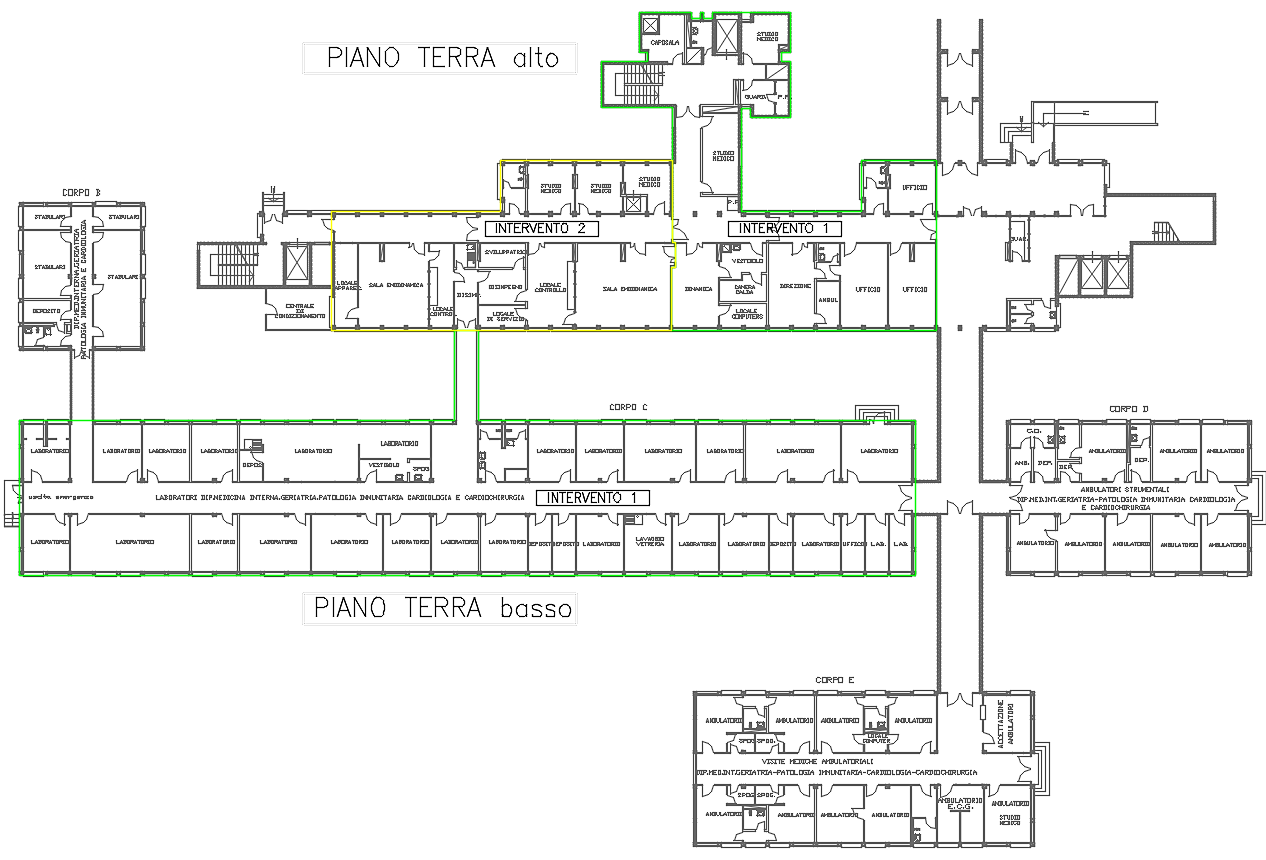
\includegraphics[width=\textheight]{6_2_cap/img/piano_terra}	
\end{sidewaysfigure}

L'edificio 2 preserva tutte le opere edili e impiantistiche realizzate all'epoca della sua costruzione. Non è difficile dedurre, quindi, che allo stato attuale sia i comportamenti estivi e invernali dell'involucro come le efficienze termo-meccaniche dell'impianto idro-aeraulico siano quantomeno inferiori a quelli consigliati dalla norma attuale vigente. 

%\begin{itemize}
%	\item componenti opachi
%	\item componenti trasparenti
%	\item ponti termici???
%	\item definizione dei vari locali
%\end{itemize}
%Metti i risultati con tabelle. 
%Inserisci foto in bianco e nero di alcuni componenti finestrati o criticità.
%Prendi in considerazione l'idea di inserire planimetrie da stampare su A3 da piegare all'interno della tesi. 
\section{L'involucro}
L'involucro dell'Edificio 2 non è cambiato in questi anni quindi non ci sono differenze con le stratigrafie indicate dall'\tit{Ing.}{Corrado Beguinot}.

Si passa ora a descrivere i componenti (opachi e trasparenti) utilizzati come dati di input per il calcolo del fabbisogno energetico e del carico termico (estivo e invernale) dell'edificio stesso.
\subsection{Componenti opachi}
\subsubsection{MURO EXT}
È il componente esterno delle facciate maggiori del Corpo A. È caratterizzato esternamente da blocchi di silicalcite alternati dagli infissi.\\La stratigrafia\\Comportamento termico. Verticalmente è caratterizzato da una diversa stratigrafia. Si è poi effettuata una media ponderale in modo tale da valutare una caratteristica termica fittizia che sia però l'espressione del comportamento della facciata.
\subsubsection{MURO EXT2}
È il componente esterno delle scale e del torrino.
\subsubsection{MURO EXT3}
È il componente esterno dei corpi bassi ovvero del Corpo B, C, D ed E.
\subsubsection{COPERTURA 1}
È la copertura del Corpo A.
\subsubsection{COPERTURA 2}
È la copertura dei Corpi B, C, E ed E.
\subsubsection{PAVIMENTO}
È il componente opaco utilizzato per modellare i pavimenti dell'Edificio 2 (quindi in comune tra tutti i corpi).
\subsection{Componenti trasparenti}
\subsubsection{FINESTRA P}
Finestra Piccola
\subsubsection{FINESTRA G}
Finestra Grande
\subsubsection{FINESTRA LUC}
Lucernario in alto in ogni blocco
\subsubsection{FINESTRA...}
Finestra 
\subsection{Definizione locali (norma 10339)}
\section{L'impianto}
\section{I risultati energetici}
\subsection{Stagione Estiva}
Inserisci sia le variazioni dei carichi termici e dell'indice di prestazione energetica.
\subsection{Stagione Invernale}
